\section{Agent, Replay, and Gateway Evaluation}

\subsection{Live trace generation and admission}

We separate live trace generation from enforcement causality. A credentialed model runtime generated action attempts in a bounded synthetic environment. The certified cohort contains \LiveTraces{} eligible traces with no model error or refusal recorded in the cohort. We freeze the resulting action traces and compare treatments through strict replay, avoiding model nondeterminism in the paired evidence.

The cohort covers synthetic prompt-injection propagation, synthetic credential and tool misuse, and a frozen benign metadata-write workflow. Eligibility is established from the captured action opportunity rather than from a model refusal or safe early termination.

\subsection{Strict replay and timing}

Each strict replay presents the same captured agent-action sequence, local policy, strategy, gateway configuration, and receiver-local monitor conditions to local-only and TCOP treatments. The controlled difference is whether and when accepted signed runtime evidence is available. A replay records evidence receipt, local correlation, local decision change, gateway outcome, and the affected agent-action opportunity.

The strict replay matrix contains \LiveReplayPairs{} paired comparisons. Figure~\ref{fig:replay-timing} reports action-relative placements. Early and boundary placements represent the tested preauthorization region; later placements can affect only later opportunities. The complete treatment table and normalized timing summary retain their denominators in Appendix~\ref{app:extended-results}.

\begin{figure*}[t]
\centering
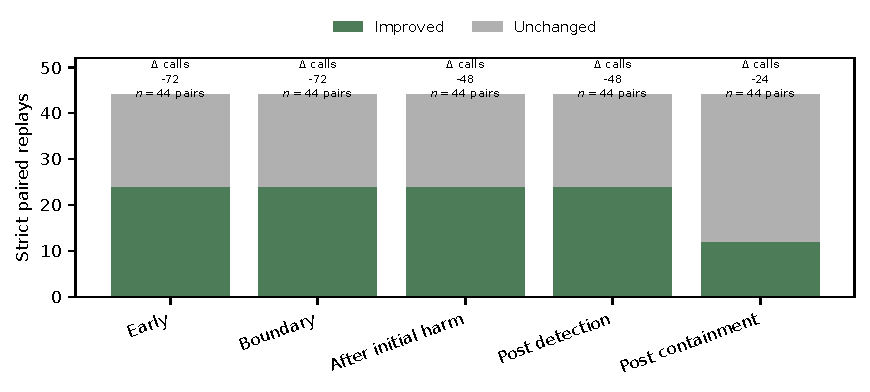
\includegraphics[width=\textwidth]{live-replay-treatments}
\caption{Strict replay results by action-relative delivery placement. Early and boundary treatments share the tested discrete preauthorization region.}
\label{fig:replay-timing}
\end{figure*}

\subsection{Post-denial substitution replay}

The separately rooted post-denial substitution study compares receiver-local strategies through the same TCOP acceptance boundary. It holds \AdaptiveStrictEpisodes{} policy-conditioned replay episodes fixed across \AdaptiveInitialBlocked{} frozen traces per policy. Every imported-evidence policy blocks the initial exact-bound action; \AdaptiveEligibleHarmfulBranches{} traces then have an eligible harmful capability, session, or delegation substitution. Exact Binding (C2) permits all \AdaptiveCTwoPostDenialCompleted{} substitutions, whereas Arrival Guard (C1), Campaign Correlation (C2E), and Standing Guard (C3) block them. Campaign Correlation uses a predeclared receiver-local relation, not a sender-provided enforcement field. Each imported-evidence strategy forwards all \AdaptiveBenignFallbacks{} of \AdaptiveBenignFallbacks{} exercised predeclared safe fallback actions. These safe fallbacks are a distinct in-campaign benign-continuation branch that the frozen policies explicitly forward after the initial denial. They are not the same-risk outside-campaign benign population on which the frontier measures Arrival Guard and Standing Guard collateral restriction.

The study also retains \AdaptiveLiveEpisodes{} bounded reference-runtime episodes. The runtime follows a predeclared harmful substitution branch after denial in \AdaptiveLiveAdapted{} episodes and a safe fallback in \AdaptiveLiveDidNotAdapt{} episodes. These runtime observations establish branch representability in the evaluated environment. The strict replay supplies the policy-conditioned conformance result; neither component estimates behavior prevalence in deployment.

\paragraph{Campaign Correlation strategy frontier:}
The separately sealed frontier evaluates \FrontierEpisodes{} deterministic policy episodes over \FrontierHarmfulAttempted{} harmful and \FrontierBenignAttempted{} benign logical actions. Its composition is fixed before policy execution (Table~\ref{tab:c2e-frontier-composition}): exact-bound and non-exact harmful actions share the \texttt{sensitive-write} risk family; the latter carry a receiver-established session-lineage relation. The same-risk benign actions outside a campaign retain that risk family but have a receiver-local campaign miss. Arrival Guard and Standing Guard block the same harmful population but constrain \FrontierCOneBenignConstrained{} and \FrontierCThreeBenignConstrained{} benign actions; Exact Binding blocks only \FrontierCTwoHarmfulBlocked{} harmful actions. Campaign Correlation blocks all \FrontierCampaignHarmfulBlocked{} campaign-linked non-exact harmful substitutions and forwards all \FrontierOutsideCampaignBenignForwarded{} benign same-risk actions outside the campaign. The receiver policy contract permits a declared delegation edge, but this frontier exercises session lineage only. Invalid, expired, and replayed context is rejected. Valid sender-suggested-only context is monitor-only, and the study records \FrontierUnrelatedRestrictions{} unrelated restrictions.

\begin{table}[t]\centering\scriptsize
\caption{Receiver-local strategy frontier. The same 10 harmful and 20 benign logical actions are evaluated per policy; this is a deterministic reference-policy result.}
\begin{tabular}{@{}p{0.48\columnwidth}cc@{}}\toprule
Strategy & \shortstack{Harmful\\blocked} & \shortstack{Benign\\constrained} \\ \midrule
Local Only (C0) & \FrontierCZeroHarmfulBlocked/\FrontierHarmfulAttempted & \FrontierCZeroBenignConstrained/\FrontierBenignAttempted \\
Arrival Guard (C1) & \FrontierCOneHarmfulBlocked/\FrontierHarmfulAttempted & \FrontierCOneBenignConstrained/\FrontierBenignAttempted \\
Exact Binding (C2) & \FrontierCTwoHarmfulBlocked/\FrontierHarmfulAttempted & \FrontierCTwoBenignConstrained/\FrontierBenignAttempted \\
Campaign Correlation (C2E) & \FrontierCTwoEHarmfulBlocked/\FrontierHarmfulAttempted & \FrontierCTwoEBenignConstrained/\FrontierBenignAttempted \\
Standing Guard (C3) & \FrontierCThreeHarmfulBlocked/\FrontierHarmfulAttempted & \FrontierCThreeBenignConstrained/\FrontierBenignAttempted \\ \bottomrule
\end{tabular}\label{tab:c2e-frontier}\end{table}


\begin{table}[t]\centering\scriptsize
\caption{Campaign Correlation frontier input composition (artifact identifier C2E). The fixed population contains five traces in each principal scenario; session lineage is the only strong relation exercised in this frontier.}
\begin{tabular}{@{}p{0.52\columnwidth}rr@{}}\toprule
Fixed trace class & Harmful & Benign \\ \midrule
Exact-bound action & \FrontierExactBindingHarmful & 0 \\
Non-exact action with receiver session lineage & \FrontierLineageHarmful & 0 \\
Predeclared safe fallback after relation & 0 & \FrontierSafeFallbackBenign \\
Same-risk action outside campaign & 0 & \FrontierOutsideCampaignBenign \\
Unrelated subject, session, or resource & 0 & \FrontierUnrelatedBenign \\
Invalid relation & 0 & \FrontierInvalidRelationControls \\
Expired relation & 0 & \FrontierExpiredRelationControls \\
Replayed relation & 0 & \FrontierReplayedRelationControls \\
Sender-suggested-only relation & 0 & \FrontierSenderSuggestedRelationControls \\ \bottomrule
\end{tabular}\label{tab:c2e-frontier-composition}\end{table}


\begin{figure}[t]
\centering
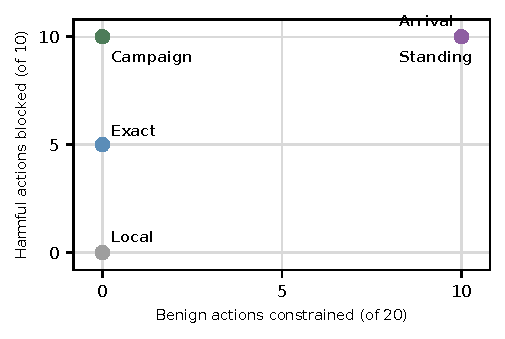
\includegraphics[width=0.94\columnwidth]{c2e-policy-frontier}
\caption{Receiver-local policy frontier in the sealed deterministic Campaign Correlation study. Arrival Guard and Standing Guard overlap at 10 benign actions constrained and 10 harmful actions blocked. The plotted points characterize configurable receiver strategies, not a mandatory TCOP response.}
\label{fig:c2e-policy-frontier}
\end{figure}

\subsection{Single-environment reference-path deployment}

The single-environment reference path runs \texttt{tcopd}-A, signed exchange, \texttt{tcopd}-B, the evaluator, and MCP gateway as separate processes on one host. It evaluates neither multi-host nor administrative separation. The \PhysicalFederationExchanges{} signed exchanges traverse both endpoints. Figure~\ref{fig:physical} separates prospective blocking from completed calls and later blocked opportunities. Each arm is one complete execution; harmful call attempts and signed exchanges are separate accounting units. Every gateway block cites Domain-B-local policy and decision provenance, establishing composition of this reference path.

\begin{figure}[t]
\centering
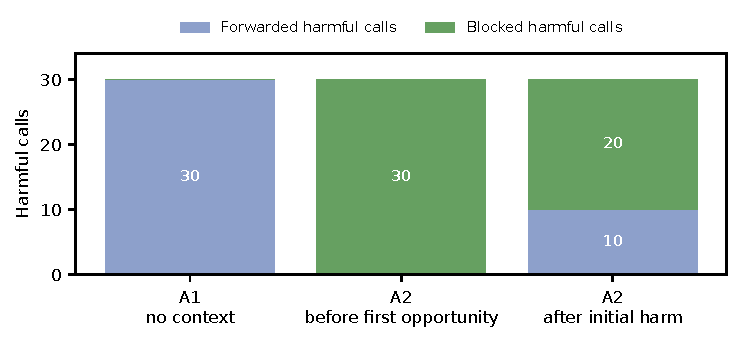
\includegraphics[width=\columnwidth]{physical-timing}
\caption{Single-environment reference-path timing result. The late arm separates already forwarded harmful calls from subsequent calls blocked by a Domain-B-local decision.}
\label{fig:physical}
\end{figure}

\begin{table}[t]\centering\small
\caption{Single-environment reference-path gateway arms. Each block is attributable to a Domain-B-local decision.}
\begin{tabular}{@{}p{0.40\columnwidth}rr@{}}\toprule
Arm & Forwarded & Blocked \\ \midrule
A1, no context & \AOneForwarded & 0 \\
A2, before first opportunity & 0 & \EarlyBlocked \\
A2, after initial harm & \LateForwarded & \LateBlocked \\ \bottomrule
\end{tabular}\label{tab:physical}\end{table}


\subsection{Measured scope}

The reported sub-millisecond values characterize the local deterministic harness. The single-environment reference-path deployment establishes that the tested relay, evaluator, and gateway adapter compose; strict replay supplies the controlled counterfactual. The timing treatments vary delivery relative to a receiver-local authorization boundary in synthetic action sequences. They do not reconstruct or draw measurements from a public incident.
